% !TeX spellcheck = en_US
\documentclass[winfonts]{njuthesis}
%%%%%%%%%%%%%%%%%%%%%%%%%%%%%%%%%%%%%%%%%%%%%%%%%%%%%%%%%%%%%%%%%%%%%%%%%%%%%%%
% 设置论文的中文封面
% 论文标题
\title{基于超声波和IMU的室内定位系统}
% 论文作者姓名
\author{陈勇虎}
% 论文作者学号
\studentid{161240005}
% 导师姓名职称
\supervisor{谢磊}
% 导师职称
\supervisortitle{副教授}
% 论文作者院系
\department{匡亚明学院}
% 论文作者专业方向
\major{计算机科学与技术}
% 论文作者的年级
\grade{2016级}
% 论文提交日期,需设置年、月、日。此属性可选,默认值为最后一次编译时的日期,精确到日。
\submitdate{2020年5月20日}

%%%%%%%%%%%%%%%%%%%%%%%%%%%%%%%%%%%%%%%%%%%%%%%%%%%%%%%%%%%%%%%%%%%%%%%%%%%%%%%
% 设置论文的英文封面
% 论文的英文标题
\englishtitle{IMU}
% 论文作者姓名的拼音
\englishauthor{Yonghu Chen}
% 导师姓名职称的英文
\englishsupervisor{Professor Lei Xie}
% 论文作者所在院系的英文名称
\englishdepartment{School of Computer Science}
% 论文作者所在学校或机构的英文名称。此属性可选,默认值为``Nanjing University''。
\englishinstitute{Nanjing University}
% 论文完成日期的英文形式,默认最后一次编译的时间
\englishdate{May 20, 2020}
% 专业
\englishinstitute{Computer Science and Technology}

%%%%%%%%%%%%%%%%%%%%%%%%%%%%%%%%%%%%%%%%%%%%%%%%%%%%%%%%%%%%%%%%%%%%%%%%%%%%%%%
% 设置论文的页眉页脚
\usepackage{fancyhdr}
\pagestyle{fancy}
%\lhead{\bfseries 141180092 }
\chead{毕业论文}
\rhead{陈勇虎}
%\lfoot{From: K. Grant}
%\cfoot{To: Dean A. Smith}
%\rfoot{\thepage}
\renewcommand{\headrulewidth}{0.4pt}
%\renewcommand{\footrulewidth}{0.4pt}

%%%%%%%%%%%%%%%%%%%%%%%%%%%%%%%%%%%%%%%%%%%%%%%%%%%%%%%%%%%%%%%%%%%%%%%%%%%%%%%
\begin{document}
% 制作中文封面
\maketitle
% 制作英文封面
% \makeenglishtitle
% 毕业论文过程管理四页表
\controlpage %可以将word文件交给老师签字后扫描转成pdf,然后命名为controlpage.pdf

% 论文的中文摘要
\begin{abstract}


基于IMU和智能手机的室内定位系统

% 同时应该注意到,空白页是故意留白,以便章节开头能够出现在偶数页。
% 中文关键词。关键词之间用中文全角分号隔开,末尾无标点符号。
\keywords{IMU; 智能手机; }
\end{abstract}

%%%%%%%%%%%%%%%%%%%%%%%%%%%%%%%%%%%%%%%%%%%%%%%%%%%%%%%%%%%%%%%%%%%%%%%%%%%%%%%
% 论文的英文摘要
\begin{englishabstract}
IMU
% 英文关键词。关键词之间用英文半角逗号隔开,末尾无符号。
\englishkeywords{IMU, smart phone, }
\end{englishabstract}

%%%%%%%%%%%%%%%%%%%%%%%%%%%%%%%%%%%%%%%%%%%%%%%%%%%%%%%%%%%%%%%%%%%%%%%%%%%%%%%
% 论文的前言,应放在目录之前,中英文摘要之后
%
%\begin{preface}
%
%在过去的40年中,手写中文文本领域识别(HCTR)取得了很大的进展[1,2]。
%
%\vspace{1cm}
%\begin{flushright}
%饶安逸\\
%2018年5月15日于南大仙林
%\end{flushright}
%
%\end{preface}

%%%%%%%%%%%%%%%%%%%%%%%%%%%%%%%%%%%%%%%%%%%%%%%%%%%%%%%%%%%%%%%%%%%%%%%%%%%%%%%
% 生成论文目录
\tableofcontents

%%%%%%%%%%%%%%%%%%%%%%%%%%%%%%%%%%%%%%%%%%%%%%%%%%%%%%%%%%%%%%%%%%%%%%%%%%%%%%%
% 生成插图清单。如无需插图清单则可注释掉下述语句。
%\listoffigures

%%%%%%%%%%%%%%%%%%%%%%%%%%%%%%%%%%%%%%%%%%%%%%%%%%%%%%%%%%%%%%%%%%%%%%%%%%%%%%%
% 生成附表清单。如无需附表清单则可注释掉下述语句。
%\listoftables

%%%%%%%%%%%%%%%%%%%%%%%%%%%%%%%%%%%%%%%%%%%%%%%%%%%%%%%%%%%%%%%%%%%%%%%%%%%%%%%
% 开始正文部分
\mainmatter

%%%%%%%%%%%%%%%%%%%%%%%%%%%%%%%%%%%%%%%%%%%%%%%%%%%%%%%%%%%%%%%%%%%%%%%%%%%%%%%
% 学位论文的正文应以《绪论》作为第一章
\chapter{绪论}\label{chapter_introduction}
	\section{研究背景及意义}
		在室内环境(办公室,住所)中想要寻找一个小物品,诸如钥匙,硬币,可以说是一件令人费神的事情了\cite{HyperEarAbstract}。在游戏世界和虚幻的电影场景中,我们都或多或少接触过类似于“寻宝罗盘”的神奇宝物,它可以类似一个掌上的指南针,时刻指示“宝物”的方向。随着各式各样移动智能设备的广泛涌现,例如智能手机,智能手表,这些设备不仅自带了诸多传感器,同时可以为用户提供很好的UI界面。因此,如果可以利用这些设备实现类似于寻宝罗盘的功能,用于寻找我们室内环境中的小物品,无疑是有趣且富有创造性的。
		
		随着对位置精度要求的提高,对于定位技术的研究也越加深入。传统的全球定位系统(Global Positioning System,GPS)\cite{wikipedia_GPS}是现代定位系统的首选,然而,在室内环境中,由于卫星信号受到建筑物的削弱,遮蔽,以及在复杂的室内环境下引起的信号反射,折射,透射等造成的多径和非视距传输现象, 导致定位误差较大,所以卫星定位的精度已经无法满足室内定位的需求,因此以无线传感网为媒介的定位系统逐渐发展起来。
		
		
	
	\section{国内外研究现状}
		\subsection{室内定位方案}

	\section{研究内容与本文主要工作}

		\begin{enumerate}
		\item
			
		\item
			
		\item 
			
		\end{enumerate}

	\section{论文的整体结构}
		本文的各章节组织结构如下:
		
		第一章:绪论
		
		第二章:相关工作
		
		第三章:实验
		
		第四章:总结与讨论
		
		。。。

%%%%%%%%%%%%%%%%%%%%%%%%%%%%%%%%%%%%%%%%%%%%%%%%%%%%%%%%%%%%%%%%%%%%%%%%%%%%%%%
\chapter{声源定位相关研究工作}
	\section{声源定位方案}
	
		在现代城市中,利用机器视觉实现的机器人导航系统已是非常普遍。然而由于机器视觉本身存在的问题,使得利用机器视觉进行机器人导航在一些环境下表现的差强人意,比如,在光线不足的情况下,或者是在机器人的“视野”所不能到达的地方,机器人就找不到目标在空间中的位置,如果给机器人安装上“耳朵”,给予机器人声源采集装置,在进行人机交互的时候,人就可以通过语音告诉机器人自己现在所处的位置,机器人对声源信号进行处理,求解出声源的具体位置,然后制定关节运动决策,使交互对象重新进入其视野之内。
		
		\subsection{声源定位技术的应用}
		\subsection{远程视频会议及远程教学等}
	
	\section{室内定位的信道模型}
	
		
		
		\subsection{基于RSS的信道模型}
		
		
		
		\subsection{基于TOA的信道模型}
		
		
		
		\subsection{基于TDOA的信道模型}
		
		
		
		\subsection{射线跟踪信道模型}
	
	\section{室内定位为技术原理}
		\subsection{几何定位法}
			\subsubsection{多边测距法}
			
			
			\subsubsection{双曲线定位法}
			
			
			
			\subsubsection{三角定位法}
		\subsection{场景分析法}

%%%%%%%%%%%%%%%%%%%%%%%%%%%%%%%%%%%%%%%%%%%%%%%%%%%%%%%%%%%%%%%%%%%%%%%%%%%%%%%	
\chapter{智能手机的感知和识别}\label{chapter_mobile}
	\section{双麦克风的节点定位}
		
		近些年来,基于声学传感器的定位系统越来越受到人们的关注,依赖于多个同步的麦克风,采集到的多路同步信号,用以后续的信号处理。随着无线传感网的不断发展进步,无线传感网定位问题也是一个比较热门的课题。而节点定位作为目标定位的前提条件,节点的定位精度也影响着目标定位的结果。然而,尽管目前有很多节点定位算法,但是因为功耗,成本等客观条件的限制,这些定位算法在很多场景中并不能很好的应用。
		
		随着可移动智能设备的普及,尤以智能手机更为常见。自2018年起,大部分的智能手机都开始集成两个甚至多个麦克风,除了底部的通话话筒以外,智能手机的顶部都还有一个“小孔”(不同的手机可能有所区别,例如iPhone手机的次麦克风可能位于主摄像头的附近)(如图\ref{fig:iphone-dual-microphone}),这就是手机的降噪麦克风,它的主要作用是实现有噪声环境下的高质量通话。
		
		\begin{figure}[htbp]
			\centering
			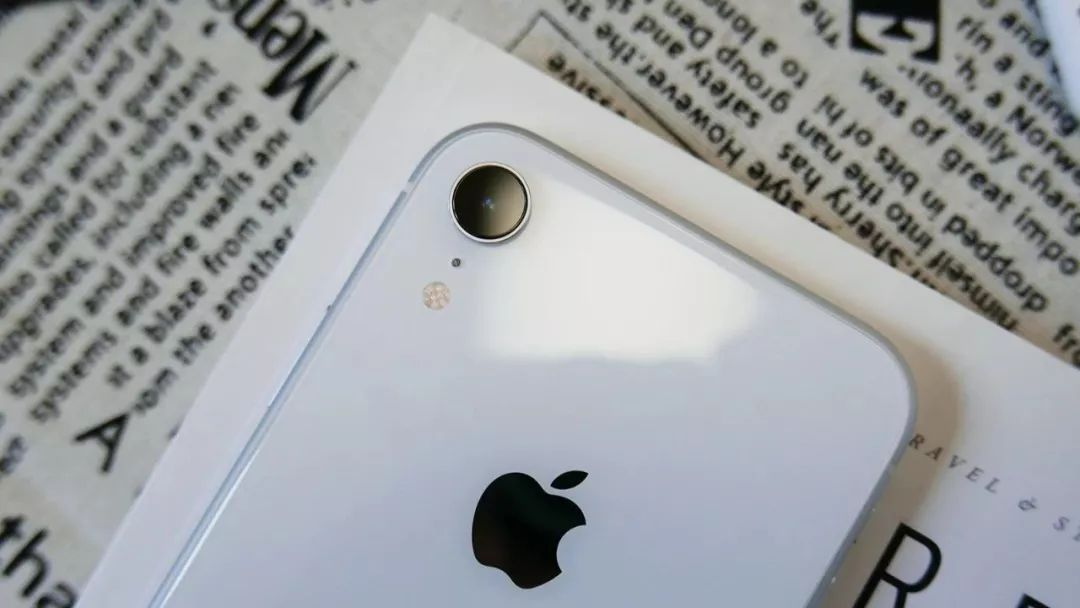
\includegraphics[width=0.7\textwidth]{iPhone-dual-micphone.jpeg} 
			\caption{iPhone8的次麦克风手机位于摄像头附近}
			\label{fig:iphone-dual-microphone}
			%\vspace{0.8cm} % 用来调整和下方文字的间距
		\end{figure}
	
		手机上设有的两个电容式麦克风尽管作用不同,但是其性能相同,对声音信号的收集能力相同。利用双麦克风系统的时间同步(两个麦克风是集成于同一个设备的,因此完全时钟同步)特性,即使两个麦克风(如图\ref{fig:samsung-dual-microphone})之间的距离较短(16cm左右,不同手机略有差异),也可以根据声音到达两个麦克风时刻的差异计算TDOA,因此,利用双麦克风系统手机结点作为实验设备有效解决了研究过程中时钟同步的问题。
		
		\begin{figure}[htbp]
			\centering
			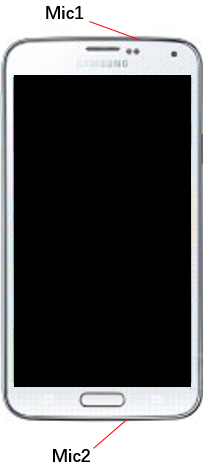
\includegraphics[height=0.35\textheight,width=0.3\textwidth]{samsung-dual-microphone.png} 
			\caption{Dual-microphone phone}
			\label{fig:samsung-dual-microphone}
			%\vspace{0.8cm} % 用来调整和下方文字的间距
		\end{figure}
	
		目前已经有很多利用双麦克风结点实现声源定位或者其他有趣的研究成果。例如利用双麦克风智能手机进行手势轨迹感知\cite{VSkin};Aarab 使用双麦克风节点定位的思路测算说话人的位置\cite{DMArrays}。
		
	\section{智能手机的传感器}
	
		随着技术的进步,手机已经不再是一个简单的通信工具,而是具有综合功能的便携式电子设备。大多数的Android设备都有内置传感器,用来测量运动,环境变化等。例如重力传感器可以用来推断用户的手势和动作,温度传感器等可以用来探测环境,地磁传感器等可以用来指示方向。
		
		\subsection{加速计传感器}
		
		
			
		\subsection{陀螺仪}
		\subsection{重力传感器}
		\subsection{磁力计}

%%%%%%%%%%%%%%%%%%%%%%%%%%%%%%%%%%%%%%%%%%%%%%%%%%%%%%%%%%%%%%%%%%%%%%%%%%%%%%%
\chapter{基于双麦克风手机的声源定位}\label{chapter_work}
	近些年来,智能手机已经成为人们生活中不可缺少的一部分,手机上集成的传感器的发展,使得智能手机的功螚越来越强大。在前面我们已经简述到大部分智能手机已经配备两个麦克风,用于消除我们在日常通话中的环境噪声,并且可以很好的解决的时钟同步问题。因此,利用智能手机的优势,通过获取同一个手机两个麦克风的声音数据,我们从中过滤出我们想要的声音信号,得到两路同步的声音信号,利用智能手机计算出两个麦克风的到达时间差(TODA),对TDOA信号进行后续的处理,就可以实现一些有意义的功能。
	
	。。。
	
	
	\section{数据采集}
	本文利用具有双麦克风系统的智能手机(Samsung 5)作为传感器结点的进行声音信号的手机,在分析阶段,使用MATLAB科学工具对信号进行解析显示。(TODO声音信号)
	
	。。。。
	
	下表中\ref{table:parameters-of-S5}展示了采集声音信号的手机参数,实验中使用了SamSung S5手机作为实验设备,S5集成了两个同步的麦克风,分别位于手机的底部和顶部,而这个两个麦克风的声音采集能力完全相同。目前的智能手机最高采样率都可以达到44100Hz,每秒钟就可以获得44100个声音信号的样本值。
	
	\begin{table}[htbp]
		\setlength{\belowcaptionskip}{7pt}
		\caption{SamSung S5设备参数}
		\centering
		\begin{tabular}{ccc}
			\hline 
			参数 & 描述 \\
			\hline
			灵敏度 & -26dB\\
			麦克风距离 & 12cm \\
			采样频率 & 44100Hz\\
			\hline
		\end{tabular} 
		\vspace{0.2cm}
		\label{table:parameters-of-S5}
	\end{table}

	本文利用内置双麦克风的S5手机进行实时采集声音信号,首先介绍offline处理的,对信号进行汇总处理和分析。在底层获取的声音信号实际是个一维数组,当然利用MATLAB进行读取,会转换成两个一维数组,分别代表两个麦克风的数据。在原始的底层存储中,一维数组的值即是采集的到数据。如图\ref{fig:sound-data}所示,实验中,我们采用16bit的stero的格式进行采集,因此根据图中的存储方式很容易分别获得两个麦克风的数据,并且两组数据是完全满足时钟同步的。为了环境噪声或者其他声音的干扰,本文中设置了一个基于能量的硬阈值,当每个buffer信号的能量低于该阈值时,则认为没有声源发生,当平均能量高于该阈值时,认为有声源发生,从而进行后面的处理。
	
	\begin{figure}[htbp]
		\centering
		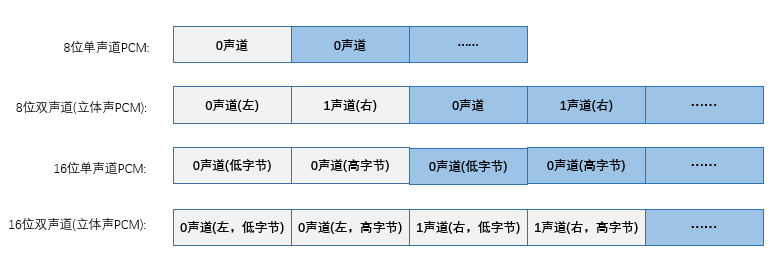
\includegraphics[scale=0.6]{sound-data.png} 
		\caption{数据存储方式}
		\label{fig:sound-data}
		%\vspace{0.8cm} % 用来调整和下方文字的间距
	\end{figure}
	
	数据采集阶段核心代码如下所示.手机条用麦克风不断检测周围环境的声音信号,当信号端的平均能量高于阈值时,系统判断声源发声,并且将两路的声音信号进行分离,用于后续的处理。
	
	\begin{algorithm}
		\caption{dual-microphone signals acquisition(双麦克风信号采集)}
		\label{alg:data-collecting}
		\begin{algorithmic}[1]
			\STATE {mAudioRecord.startRecording()}
			\STATE {//系统检测周围环境中的声音信号} 
			\WHILE{isRecording}
				\STATE {//读取两路声音信号} 
				\STATE {read = mAudioRecord.read(mBuffer, 0, BUFFER\_SIZE)}
				\IF {read <= 0}
					\STATE {return false}
				\ELSE
					\STATE {//根据设定的阈值判断是否有声源发声}
					\STATE { sum = 0}
					\FOR{$i=0$ to read} 
						\STATE {sum += Math.abs(mBbuffer[i])}
					\ENDFOR 
					\STATE {//达到设定的阈值,认为有声源发声}
					\IF{sum / read > thresholdValue}
						\STATE {//两路信号分离}
						\STATE {index = 0}
						\FOR{$i=0$ to mBuffer.length/2}
							\IF{i \% 2 == 0}
								\STATE{System.arraycopy(mBuffer, i * 2, mBuffer1, 0, 2)}
								\STATE{LY[index] = ((mBuffer1[0]\&0x000000FF) | (((int)mBuffer1[1])<<8))/ 32768.0}
								\STATE{LYList.add(LY[index])]}
								\STATE{index = i / 2}
							\ELSE
								\STATE{System.arraycopy(mBuffer, i * 2, mBuffer2, 0, 2)}
								\STATE{RY[index] = ((mBuffer2[0]\&0x000000FF) | (((int)mBuffer2[1])<<8))/ 32768.0}
								\STATE{RYList.add(RY[index])]}
							\ENDIF
						\ENDFOR
					\ENDIF					
				\ENDIF
			\ENDWHILE
		\end{algorithmic}
	\end{algorithm}
	
	
	\section{offline算法及声音信号处理}
		\subsection{信号除噪}
		\subsection{异常点移除}
		\subsection{}
		\subsection{TDOA计算}
	\section{零速校准}
	\section{offlinee到online的迁移}
	
\chapter{模型系统实现与实验分析}
	\section{开发环境与平台}
	\section{系统设计}
		\subsection{多模块设计}
		\subsection{界面与运行方式}
	\section{实验与分析}
	\section{本章小结}
%%%%%%%%%%%%%%%%%%%%%%%%%%%%%%%%%%%%%%%%%%%%%%%%%%%%%%%%%%%%%%%%%%%%%%%%%%%%%%%
\chapter{总结与展望}
	\section{工作总结}
	\section{前景展望}
%%%%%%%%%%%%%%%%%%%%%%%%%%%%%%%%%%%%%%%%%%%%%%%%%%%%%%%%%%%%%%%%%%%%%%%%%%%%%%%
\bibliography{sample}
%%%%%%%%%%%%%%%%%%%%%%%%%%%%%%%%%%%%%%%%%%%%%%%%%%%%%%%%%%%%%%%%%%%%%%%%%%%%%%%
	% 致谢
	\begin{acknowledgement}
		
		非常感谢在Dislab实验室度过的两年时光,让我在实验室里拓宽眼界的同时,也不断纠正了自己的学习方法和学习态度。我的毕业论文撰写和系统实现中,也或多或少的遇到许多困难,也走过很多弯路。我很感谢我的导师谢磊副教授,从我毕设选题阶段,到我研究工作的开展,再到最后的论文撰写中,谢老师都给予了我细心的指导和点拨,给我纠正了很多错误的方向,避免我走了很多弯路。在实验室的两年,谢磊老师也给我的研究工作不断指引方向,在此,我向谢磊老师致以最真挚的谢意。
		
		同样,我也要感谢在Dislab实验室的同一课题组的各位师兄师姐,鲁欣然师兄在我的成长道路上指引了很多,从细节方面给予我帮助,王楚豫师兄同样,给了我研究工作上的很多帮助,让我的研究工作变的富有创新,也是他们给我提出的宝贵建议,让我可以不断改进自己。
		
		感谢大学四年来四种相伴的同学和朋友,因为你们的存在,我的大学才会在忙碌中透露出精彩。感谢每一位悉心教导我的老师,感谢钱柱中教授的指引,让我能够去香港游学增长知识和阅历,让我在问题求解的课程中感受到计算机和算法的魅力。
		
	\end{acknowledgement}
%%%%%%%%%%%%%%%%%%%%%%%%%%%%%%%%%%%%%%%%%%%%%%%%%%%%%%%%%%%%%%%%%%%%%%%%%%%%%%%
\end{document}
